\chapter{Introducción}
\section{Objetivo}
Determinar ciertas características de un amplificador (Impedancia de entrada y salida; Ganancia de tensión y de potencia). Emplear instrumentos con escalas de \textbf{dB}

\section{Materiales e Instrumental necesarios}
\begin{itemize}
	\item Amplificador de baja frecuencia con fuente de alimentación.
	\item Generador de señales con salida sinusoidal.
	\item Juego de potenciómetros ajustables.
	\item Multímetro analógico con escala en dB.
	\item Osciloscopio de usos generales.
\end{itemize}

\section{Introducción}
En este trabajo práctico, el estudiante empleará métodos de medición e instrumentos sencillos para la determinación de las principales características de una red de dos puertos (básicamente un amplificador).  Los métodos  que aquí ensayaremos abarcan ideas generales de gran interés en un amplio campo de las mediciones. Se verá,  por ejemplo, la utilidad de las escalas en dB que poseen algunos instrumentos, y se implementará un método de substitución para medir una
magnitud en forma indirecta.
Para este trabajo se empleará un amplificador de baja frecuencia  que no tiene ninguna aplicación específica.
Se puede verificar el correcto funcionamiento  del amplificador midiendo las tensiones indicadas sobre las placas en los puntos de prueba preparados para ese efecto.

\begin{figure}
	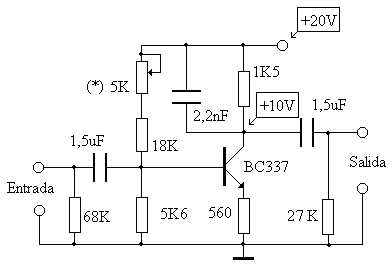
\includegraphics[width=\linewidth]{imagenes/intro1-1.png}
